\section{Machine Learning}

This section presents results obtained by application of neural networks (NNs) for performing MD simulations for two systems described in preceding chapters. The study was done by using NN model able to predict potential energy, forces and dipole moment for given geometry. This model was provided by Schnetpack~\cite{schnetpack}. For both systems considered here, the same parameters were used. The NN consisted of 3~interaction layers with 7.5~{\AA} cosine cutoff with pairwise distances expanded on 20~Gaussians and 128~atomwise features layers with convolution filters. NN was trained for 200~epochs on energies, forces and dipole moments of selected frames from classical/ab initio trajectories. For evaluation of results, mean square error loss function was used with weights for every property: 0.005 for energy, 0.005 for dipole moment and 0.99 for forces. The division of the available dataset was in every case the same: 86\% of frames were used as training set, 12\% as validation set and 2\% were left as testing set. After training, for chosen systems 35~ps of MD simulation with time step of 0.25~fs were obtained.

\subsection{Ethylene carbonate}

For neat ethylene carbonate (EC) classical MD simulations at the temperature of 400~K were performed. From these trajectories 60~000 structures containing 5~or 10~EC molecules were chosen, and for each of them energies, forces and dipole moments were calculated with PBE functional in the 6-31+G* basis set and the Grimme's dispersion correction~\cite{grimme-d3} in Gaussian~v09~\cite{gaussian}. They were used for training the NN in Schnetpack. At the end of the training the value of loss function for training set was $7.17\cdot 10^{-5}$ and for validation set $9.08\cdot 10^{-5}$.

\begin{figure}[ht]
    \centering
    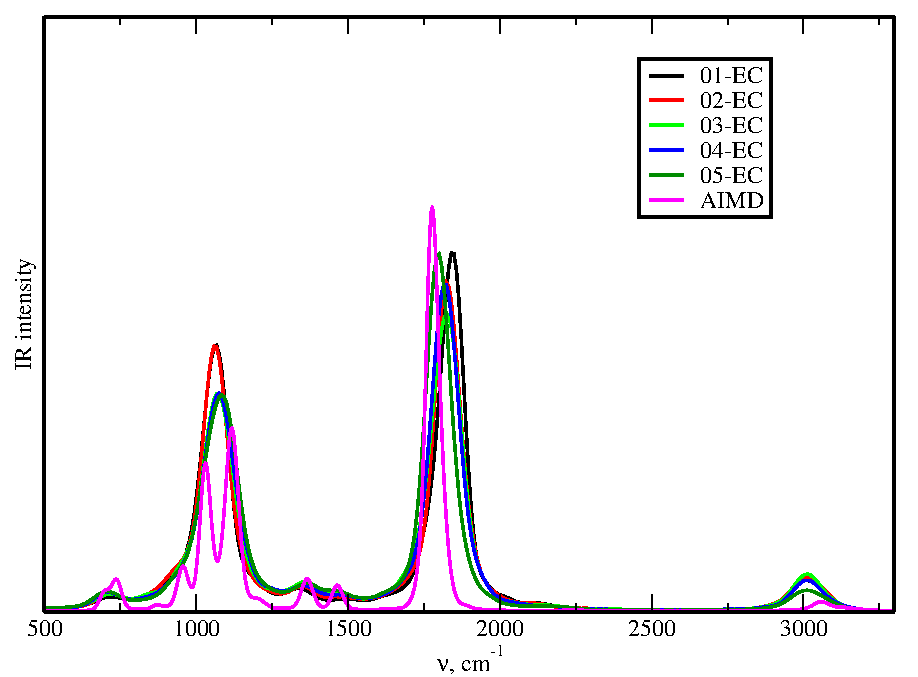
\includegraphics[width=0.6\textwidth]{img/5-alternatives-to-aimd/3-ml/ec.png}
    \caption{Infrared spectra obtained from MD simulation based on NN for systems containing 1~to~5 molecules of EC. Spectrum obtained from AIMD is shown for comparison}
    \label{fig:ml-ec}
\end{figure}

Simulations were performed for systems containing 1, 2, 3, 4 or~5 molecules of EC. For bigger number of molecules the system fell apart during the simulation. IR spectra obtained from such simulations are shown in Figure~\ref{fig:ml-ec} together with AIMD result for comparison. It could be observed that positions of bands are close to these obtained from AIMD simulation, however for vibrations with frequencies below 1800~cm$^{-1}$ number of bands obtained from NN based MD is smaller with respect to AIMD, this is especially visible for bands between 950 and 1200~cm$^{-1}$. Also frequencies of C=O and C-H stretching bands (1800~cm$^{-1}$ and about 3100~cm${-1}$ respectively) are different than in AIMD, the former is blue shifted and the latter is red shifted. The probable cause may be the difference in the basis sets and in the system size --- NN-based simulations included small number of EC molecules and were performed without PBC. Nevertheless, it is visible for C=O stretching band, that with growing number of EC molecules in the simulated system, the position of the maximum is moving towards the maximum observed in AIMD. Thus, probably better NN model not suffering from the disintegration of bigger systems would lead to almost identical spectrum as in AIMD.

\subsection{Water}

Structures of water systems containing 10, 20 or 30~molecules were obtained from the AIMD trajectories for neat water (section~\ref{section:il-h2o-structural}) and from the classical MD simulations in TIP3P~FF~\cite{tip3p-1,tip3p-2}. In the latter, additional trajectories were recorded for changed parameters of the system (density too low or too high, modified FF parameters) in order to generate some geometries distorted from the average for better training. The NN was trained on energies, forces and dipole moments calculated in Gaussian v09~\cite{gaussian} at the PBE/6-31+G* level with Grimme's dispersion correction~\cite{grimme-d3} for 50~000~structures. At the end of the training the value of loss function for training set was $1.2\cdot 10^{-4}$ and for validation set $1.77\cdot 10^{-4}$.

\begin{figure}[ht]
    \centering
    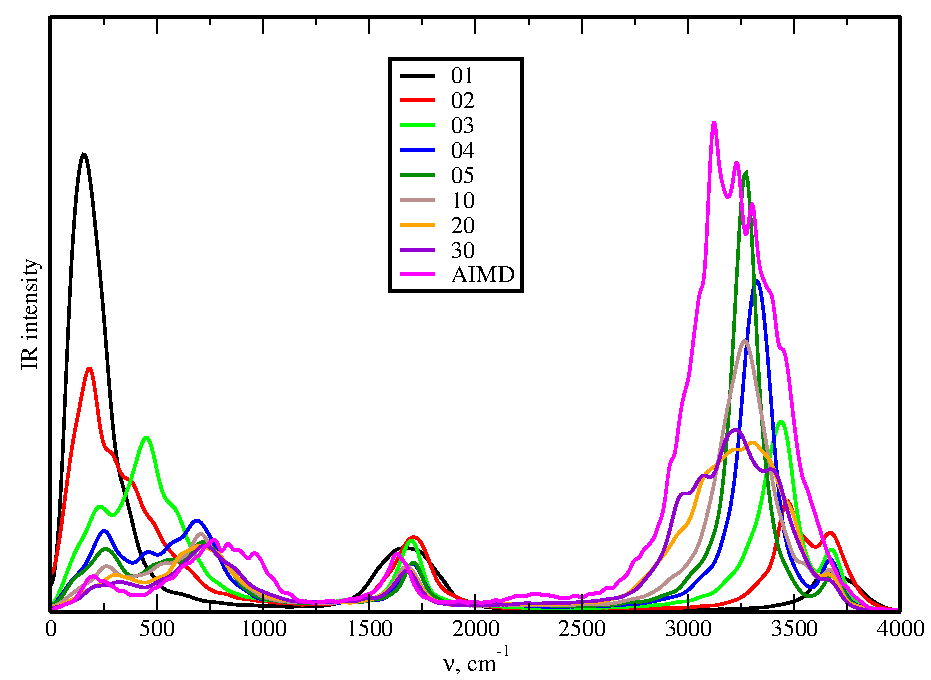
\includegraphics[width=0.6\textwidth]{img/5-alternatives-to-aimd/3-ml/h2o.png}
    \caption{Infrared spectra obtained from MD simulation based on NN for systems containing 1~to~30 molecules of water. Spectrum obtained from AIMD is shown for comparison}
    \label{fig:ml-h2o}
\end{figure}

After training the model, MD simulations were performed for systems containing 1, 2, 3, 4, 5, 10, 20 and~30 molecules of water. Obtained IR spectra, with AIMD spectrum for comparison, are shown in Figure~\ref{fig:ml-h2o}. Tendencies are similar as these observed for EC: in general, positions of bands are close to those in the spectrum obtained from AIMD with shifting their frequencies towards AIMD values with growing number of molecules used for simulation. What is more, for systems with small number of H$_2$O molecules, the O-H band is in the high frequency range of the spectrum (about 3800~cm$^{-1}$) in opposition to frequency in AIMD (about 3200~cm$^{-1}$). For system with 1~water molecule only the band at 3800~cm$^{-1}$ is present, while for systems with 2~or3~water molecules also an additional band with lower frequency appears. With growing size of the system, the band at 3800~cm$^{-1}$ is disappearing. It is also visible, that the O-H band becomes broader with increasing number of water molecules. These effects are related to the formation of hydrogen bonds and are similar to these observed for ILs mixed with H$_2$O: "free" O-H bonds have higher frequencies of stretching and the frequency becomes lower upon formation of HBs. The systematic shift of this band with growing size of the system is therefore related to growing probability of HB formation.

For this case, not only the frequencies were in a~satisfactory agreement with AIMD results, but also the effect of hydrogen bonding on the frequency of the O-H bond was reproduced.

As a~test, another NN~was trained, using for training only the data obtained from classical MD. The results of the simulation were approximately the same. Thus, in this case, structures extracted from classical MD are sufficient, without the need to use expensive AIMD to generate the geometries.

Methods for MD simulation based on the output of pre-trained NN seem to be a~promising alternative for computationally expensive AIMD. As shown here they are capable of reproduction of HB effect on the IR spectrum. However, these methods still need further investigation, because simulations for moderately large systems were unstable: in all studied cases molecules became increasingly distorted, some bonds broke and finally the system disintegrated.